\chapter{Introduction}\label{chapter:introduction}
Over the last two decades, the landscape of Computer Architecture has changed radically from sequential to parallel . Due to the limiting factors of technology we have moved from single core processors to multi core processors having a network interconnecting them. Traditionally, the approach of designing algorithms has been sequential, but designing algorithms in parallel is gaining more importance now to better utilize the computing power available at our disposal. Another important trend that has changed the face of computing is an enormous increase in the capabilities of the networks that connect computers with regards to speed, reliability etc. These trends make it feasible to develop applications that use physically distributed resources as if they were part of the same computer. A typical application of this sort may utilize processors on multiple remote computers, access a selection of remote databases, perform rendering on one or more graphics computers, and provide real-time output and control on a workstation. Computing on networked computers ("Distributed Computing") is not just a subfield of parallel computing as the basic task of developing programs that can run on many computers at once is a parallel computing problem. In this respect, the previously distinct worlds of parallel and distributed computing are converging.\\ \par
\noindent
As technology advances, we have newer problems or applications that demand larger computing capabilities which push the limits of technology giving rise to newer advancements. The performance of a computer depends directly on the time required to perform a basic operation and the number of these basic operations that can be performed concurrently. A metric used to quantify the performance of a computer is FLOPS (floating point operations per second). The time to perform a basic operation is ultimately limited by the "clock cycle" of the processor, that is, the time required to perform the most primitive operation. The term \textbf{\textit{High Performance Computing (HPC)}} refers to the practice of aggregating computing power (multiple nodes with processing units interconnected by a network in a certain toplogy) or the use of parallel processing for running advanced application programs efficiently, reliably and quickly. The term applies especially to systems that function above a \textbf{\textit{teraflop}} or \textbf{\textit{$10^{12}$}} floating-point operations per second. The term HPC is occasionally used as a synonym for Supercomputer that works at more than a \textbf{\textit{petaflop}} or \textbf{\textit{$10^{15}$}} floating-point operations per second. The most common users of HPC systems are scientific researchers, engineers, government agencies including the military, and academic institutions. In general, HPC systems can refer to Clusters, Supercomputers, Grid Computing etc. and they are usually used for running complex applications.\\ \par
\noindent
A \textbf{\textit{Batch System}} is used to manage the resources in a HPC System. It is a middleware that comprises of two major components namely the \textbf{\textit{Resource Manager}} and \textbf{\textit{Scheduler}}. The role of a Resource Manager is to act like a glue for a parallel computer to execute parallel jobs. It should make a parallel computer as easy to use as a Personal Computer (PC). A programming model such as \textbf{\textit{Message Passing Interface (MPI)}} for programming on distributed memory systems would typically be used to manage communications within a parallel program by using the MPI library functions. A Resource Manager allocates resources within a HPC system, launches and otherwise manages Jobs. Some of the examples of widely used open source as well as commercial resource managers are \textbf{\textit{SLURM, TORQUE, OMEGA, IBM Platform LSF}} etc. Together with a scheduler it is termed as a Batch System. The role of a job scheduler is to manage queue(s) of work when there is more work than resources. It supports complex scheduling algorithms which are optimized for network topology, energy efficiency, fair share scheduling, advanced reservations, preemption, gang scheduling (time-slicing jobs) etc. It also supports resource limits (by queue, user, group, etc.). Many batch systems provide both resource management and job scheduling within a single product (e.g. LSF) while others use distinct products(e.g. Torque Resource Manager and Moab Job Scheduler). Some other examples of Job Scheduling Systems are \textbf{\textit{LoadLeveler, OAR, Maui, SLURM etc.}}\\ \par
\noindent
Existing Batch Systems usually support only static allocation of resources to an application before they start which means the resources once allocated are fixed for the lifetime of the application. The complexity of applications have been growing, However, especially when we consider advanced techniques in Scientific Computing like \textbf{\textit{Adaptive Mesh Refinement (AMR)}} where applications exhibit complex behavior by changing their resource requirements during execution. The Batch Systems of today are not equipped to deal with such kind of complex applications in an intelligent manner apart from giving them the maximum number of resources before it starts that will result in a sheer wastage of resources leading to a poor resource utilization. In order to support such adaptive  applications at HPC centers there is an urgent need to investigate and implement extensions to existing resource management systems or develop an entirely new system. These supporting infrastructures must be able to handle the new kind of applications and the legacy ones intelligently keeping in mind that they should now be able to achieve much higher system utilization, throughput, energy efficiency etc. compared to their predecessors due to the elasticity of the applications.

\section{Invasive Computing}
The throughput of HPC Systems depends not only on efficient job scheduling but also on the type of jobs forming the workload. As defined by Feitelson, and Rudolph, Jobs can be classified into four categories based on their flexibility:
\begin{itemize}
\item \textbf{\textit{Rigid Job:}} Requires a fixed number of resources throughout its execution.
\item \textbf{\textit{Moldable Job: }} The resource requirement of the job can be molded or modified by the batch system before starting the job(e.g. to effectively fit alongside other rigid jobs). Once started its resource set cannot be changed anymore.
\item \textbf{\textit{Evolving Job: }} These kind of jobs request for resource expansion or shrinkage during their execution. Applications that use Multi-Scale Analysis or Adaptive Mesh Refinement (AMR) exhibit this kind of behavior typically due to unexpected increases in computations or having reached hardware limits (e.g. memory) on a node.
\item \textbf{\textit{Malleable Job: }} The expansion and shrinkage of resources are initiated by the batch system in contrast to the evolving jobs. The application adapts itself to the changing resource set.
\end{itemize}
The first two types fall into the category of what is called as the static allocation since the allocation of rigid and moldable jobs must be finalized before the job starts. Whereas, the last two types fall under the category of dynamic allocation since this property of expanding or shrinking evolving and malleable jobs (together termed adaptive jobs) happens at runtime. Adaptive Jobs hold a strong potential to obtain high system performance. Batch systems can substantially improve the system utilization, throughput and response times with efficient shrink/expand strategies for running jobs that are adaptive. Similarly, applications also profit when expanded with additional resources as this can increase application speedup and improve load balance across the job\textquotesingle s resource set.\\ \par
\noindent
Invasive Computing is a novel paradigm for the design and resource-aware programming of future parallel computing systems. It enables the programmer to write efficient resource aware programs. This approach can be used to allocate, execute on and free resources during execution of the program. The result is an adaptive application which can expand and shrink in the number of its resources at runtime. HPC infrastructures like clusters, supercomputers execute a vast variety of jobs, majority of which are parallel applications. These centers use intelligent resource management systems that should not only perform tasks of job management, resource management and scheduling but also satisfy important metrics like higher system utilization, job throughput and responsiveness. Traditionally, MPI applications are executed with a fixed number of MPI processes but with Invasive MPI they can evolve dynamically at runtime in the number of their MPI processes. This in turn supports advanced techniques like AMR where the working set size of applications change at runtime. Such kind of adaptive programming paradigms need to be complemented with intelligent resource management systems that can  achieve much higher system utilization, energy efficiency, throughput etc. compared to their predecessors due to elasticity of the applications.\par
\noindent
\\Under the collaborative research project funded by the \textbf{German Research Foundation (DFG)} in the \textbf{Transregional Collaborative Research Centre 89 (TRR89)}, research efforts are being made to investigate this Invasive Computing approach at different levels of abstraction right from the hardware up to the programming model and its applications. \textbf{Invasive MPI} is an effort towards invasive programming with MPI where the application programmer has MPI extensions available for specifying at certain safe points in the program, the possibility of a changing the resource set of the application during runtime.\\ \par

\section{Dynamic Resource Management}
Two of the most widely used resource managers on HPC systems are \textbf{SLURM} and \textbf{TORQUE}. The two major components in general of any sophisticated resource manager are the batch scheduler and the process manager. The Process Manager is responsible for launching the jobs on the allocated resources and managing them throughout their lifetime. Examples of process manager are \textbf{\textit{Hydra, SLURM Daemon (slurmd)}} etc. The process managers interact with the processes of a parallel application via the \textbf{Process Management Interface (PMI)}. In order to support Invasive Resource Management, The following components will be implemented: \textbf{\textit{iScheduler}} (Batch Scheduler for Invasic Jobs) built as an extension into an existing batch system and \textbf{\textit{iDRScheduler}} (Invasive Distributed Run TIme Scheduler) similar to a controller daemon which will sit between the batch scheduler and the process manager. \textbf{SLURM} is the choice of an existing batch system on which this prototype will be implemented for demonstrating Invasive Computing and \ref{fig:1} shows a high level illustration of the architecture for such an Invasive Resource Management.\\ \par
\begin{figure}[!htbp]
\centering
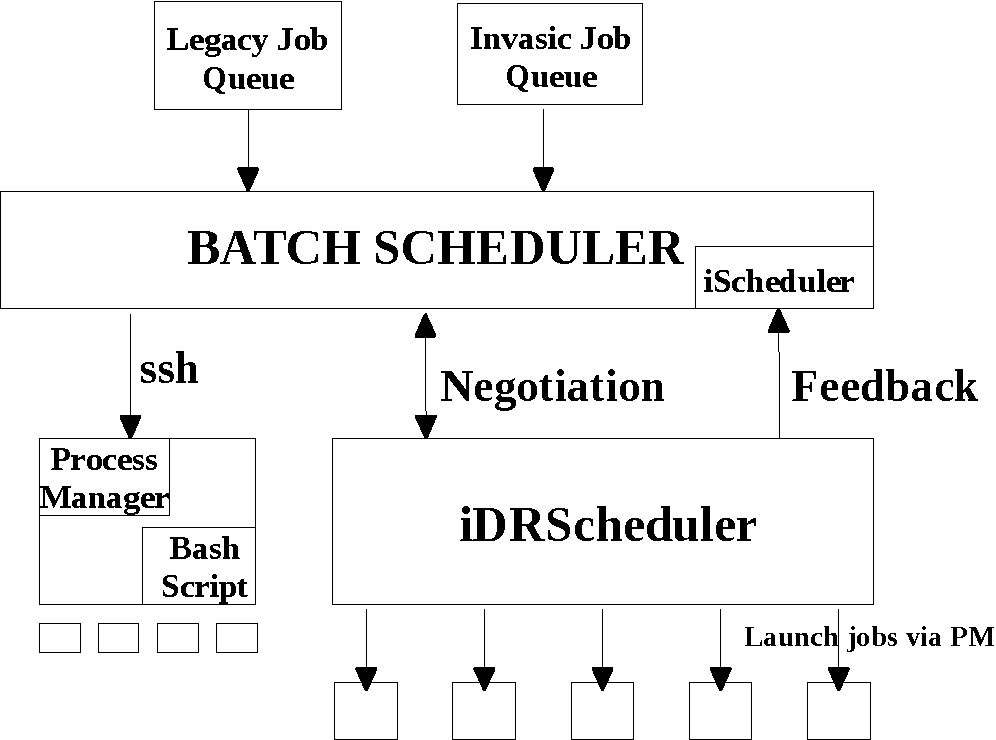
\includegraphics[width=0.8\textwidth, height=60mm]{./figures/architecture.pdf}
\caption{Invasive Resource Management Architecture}
\label{fig:1}
\end{figure}
\noindent
The above figure illustrates the proposed invasive resource management architecture. In addition to a job queue for legacy static jobs, we now have an additional job queue for invasic jobs. The existing batch scheduler needs to be extended in order to schedule these new type of Invasic Jobs and a new component called \textbf{\textit{Invasic Scheduler (iScheduler)}} is responsible for this. In contrast to modifying an existing system to support Invasive Resource Management, a new component called \textbf{\textit{Invasive Distributed Run Time Scheduler (iDRScheduler)}} is proposed which sits between the Batch Scheduler and Process Manager. The objective of such a multi-level approach is to avoid modifying the existing system which will be a substantially large effort and rather have an independent component that caters specifically to Invasic Jobs. It is responsible for managing the resources present in the Invasic paritition used specifically for running Invasic Jobs. With this approach, the existing Legacy Jobs can be served via the existing batch scheduler and the new Invasic Jobs can be served by via iScheduler and iDRScheduler. iDRScheduler talks to the iScheduler via a protocol called the Negotiation protocol to receive Invasic Jobs dispatched from iScheduler which it then launches for execution by performing some run time scheduling like pinning of jobs, expand/shrink etc.\\ \par
\noindent
The new components proposed in the architecture help achieve the objective of supporting dynamic resource management for invasic applications. iScheduler is responsible for scheduling Invasic Jobs. The scheduling decisions are communicated via negotiation protocol to iDRScheduler and these decisions are basically job(s) selected via a scheduling algorithm to be submitted for execution. The decisions will be made on the basis of Resource Offers sent by iDRScheduler which creates these resource offers based on the state of the partition. Upon receiving a resource offer, iScheduler will either accept it by selecting jobs from the queue that can be mapped to this offer or reject it. A Resource Offer can represent real or virtual resources because the iDRScheduler can also present a virtual view of resources in the hope of getting a mapping of jobs to offer that is more suitable to satisfy its local metrics such as resource utilization, power stability, energy efficiency etc. It can either accept or reject the mapping received from iScheduler. Similar to iDRScheduler, the iScheduler makes its decisions to optimize for certain local metrics such as high job throughput, reduced job waiting times, deadlines, priorities etc. This highlights the mismatching policies/metrics for which both the iDRScheduler and iScheduler make their decisions on and hence both will be involved in some kind of a negotiation via the protocol to reach a common agreement. iDRScheduler is an independent entity introduced with the purpose of inter-operating with existing batch systems rather than replacing them with an entirely new one. It may be possible that in the future this component will not be a separate entitiy but will be built into the batch system itself.\\ \par
\noindent
\textbf{\textit{Shrink/Expand Strategies: }}There are several strategies one may employ to tackle adaptive applications during runtime and take decisions that can lead to higher system utilisation, energy efficiency etc.:
\begin{itemize} 
\item Let us consider that at any given point of time there are some Invasic Jobs running in the system. If the parallel runtime environment is able to anticipate that in the near future, there may be a large window of free resources available because some applications may shrink according to a prediction of their scalability behavior with the help of run time profiling and collected performance data then iDRScheduler can provide a resource offer to iScheduler. This offer can specify a virtual list of nodes more than what is available in order to get a mapping of jobs. These jobs can then be shrunk and fit into the existing space of resources with the knowledge that they may be able to expand later.
\item Another scenario is where there is an anticipation of a smaller window of resources in the future because some of the currently running applications may expand. In such a case iDRScheduler will provide a resource offer to iScheduler with a virtual list of nodes smaller than what is currently available in order to get a mapping of jobs. These jobs can be then be expanded and fit into the existing space of resources with the knowledge that they may have to shrink later.
\item The third variation could be the case where the runtime anticipates the state of resources to remain the same as the current state for the near future since none of the running applications may expand or shrink. In such a scenario iDRScheduler will send a resource offer that is a list of nodes which is exactly the same as the available resources to iScheduler in order to get a mapping of jobs. These jobs can then be fit into the space of resources available as it is without expanding/shrinking them. 
\end{itemize}
\section{Master Thesis}
The focus of this Master Thesis is to extend the early prototype developed as a part of the guided research in the last few months. It will now give concrete meanings to the negotiation protocol, defining the format of the invasic job records, its constraints, definition of resource offers, feedback reports and most important of all to investigate and develop an efficient job scheduling algorithm at the iScheduler level. Following this closely from the Guided Research would be to continue having an automated testing in place that will help in simulating a workload of jobs, testing the job scheduling algorithm for its correctness, evaluating and analysing the performance of such a prototype for various metrics. Given below is a tentative plan of the activities proposed monthwise starting from November $15$ till May $15$ to be carried out for the duration of 6 months in this Master Thesis.\par
\subsection{Tentative Plan}
\begin{itemize}
\item Literature survey for current/recent related work on batch job scheduling from research groups focusing on problems in the areas of batch scheduling, resource management, middleware etc. In addition to this, defining resource offers, invasic job records and job constraints that can come from a pre-computed performance model of an application during its runtime or could be user defined. Once these tasks have been completed, it will follow up with extending the early prototype by the implementation of these ideas and testing them for correctness using the automated testing feature.
\item Integration of the fake iHypervisor with the real iHypervisor by making it as its plugin. Test this integration for all the earlier development using the automated testing feature for correctness. Review, analyse, fix any errors and repeate the process till the integration is stable. Follow this up by understanding the SLURM's existing scheduling algorithms including the recent Machine Learning approach for a possible reuse or enhancement. Define the format of feedback reports sent by iHypervisor and how they can be processed on the iScheduler side including its storage mechanism (possibly using SLURM's existing database functionalities). Implement these ideas in the prototype and test it thoroughly.
\item Investigate and experiment with basic scheduling algorithms first to later proceed with complex ones. Design and implement a sophisticated scheduling algorithm for mapping jobs from Invasic job queue to the resource offers sent by iHypervisor. This algorithm must perform its decision making by also using the collected history/feedback data about many statistical measures provided by iHypervisor periodically.
\item Implementation of the Job Scheduling Algorithm continues for realizing all the necessary requirements as proposed earlier till it has been successfully implemented and later followed by a lot of functional testing.
\item Test the full prototype along with the other component iHypervisor (Including its Run Time scheduling and Invasive Resource Management) for simple to complex workloads (emulating a queue of invasic jobs possibly including legacy static jobs). Testing also needs to be done with real Invasic applications developed by the \textit{Chair Of Scientific Computing}. Find issues/errors, review, analyse, correct and repeat the process till it is stable and then collect all the results necessary.
\item Coming up with the draft version of the Master Thesis Report followed by reviews, corrections. This process is repeated till the final version is decided. Also prepare the slides for the Master thesis to present them at a later stage.
\end{itemize}
\noindent
\\The above timeline highlights a tentative plan for the activities to be taken up during the Master Thesis and the $6$ items above correspond to these $6$ months of the Thesis in a chronological order. The steps may overlap or shift depending on the progress but the same overall structure will be followed for the Thesis. It will also include in parallel small amounts of documentation in the report as and when necessary during the $6$ month period and not necessarily everything at the end.\par

\section{Motivation}

\section{Document Structure}
This is end of the first section which gave an introduction to this Master Thesis and the kind of problem it deals with. The rest of this report is organized as follows:
\begin{itemize}
\item \textbf{\textit{Modeling:}} This section will explain in brief on how the DNDP will be mathematically formulated using a bilevel linear program with all its contraints, decision variables and objective function. It will explain the approach to approximate the non-linear objective function of the inner problem of DNDP which is TAP and an introduction to metaheuristics that will be used to solve such kind of a combinatorial optimization problem.
\item \textbf{\textit{Genetic Algorithm:}} This section will dive into the details of the genetic algorithm that includes all the important aspects which fall under GA that needs to be tackled in order to come up with a correct implementation yielding good performance. It will explain in detail some of the many choices one has for implementation during every step of GA.
\item \textbf{\textit{Implementation:}} This section will illustrate with the help of a flow chart the high level view of the GA implementation followed by some pseudo codes to demonstrate in a simple language the implementation details of the inner workings of GA.
\item \textbf{\textit{Experiments and Visualization:}} This section will present all the results of the experiments conducted on different types(sizes) of datasets using the implemented GA in the form of tables. It will also mention in brief some of the observations and inferences that have been drawn by looking at these results.
\item \textbf{\textit{Conclusion:}} This section concludes the report on this project with a highlight of what was successfully achieved along with the possible scope of what can be done as a part of future research work. This is followed by a list of some useful references that played an important role in the understanding of many of the concepts towards the realization of this project.
\end{itemize}
